\chapter{Dinámica semiclásica de electrones de Boch} \label{Ch:08}

En este capítulo se estudia el comportamiento de electrones en un cristal frente a campos eléctricos y magnéticos. Para ello se utiliza el formalismo clásico visto en capítulos anteriores, bajo el supuesto de que los campos externos varían suavemente en la escala del paquete de onda. La estructura de bandas de energáis $\varepsilon_n (\kn)$ se supondrá conocida.

\section{Ecuaciones del movimiento}

El paquete de ondas Bloch está constituido por funciones de odna cercanas al vector de onda $\kn$ particular. La velocidad de grupo resulta ser la expresión familiar $\vn=\D \omega / \D \kn$. Como la frecuencia asociada con una función de energía $\varepsilon$ es $\omega = \varepsilon/\hbar$ se tiene para la velocidad $\vn$ del electrón:

\begin{equation}
	\vn (\kn) = \hbar^{-1} \derivadas{\varepsilon(\kn)}{\kn} \label{Ec:08-01-01}
\end{equation}
Los efectos del cristal (potencial-periódico) sobre el movimiento de los elcetrones se contienen en la relación de dispersión $\varepsilon(\kn)$. En presencia de fuerzas externas las energías electrónica aumentará a una velocidad 

\begin{equation}
	\derivadas{\varepsilon}{t} = \Fn \cdot \vn = \frac{1}{\hbar} \Fn \cdot \derivadas{\varepsilon}{\kn}
\end{equation}
Pero por otro lado,

\begin{equation}
	\derivadas{\varepsilon}{t} = \derivadas{\varepsilon}{\kn} \cdot \derivadas{\kn}{t}
\end{equation}
Combinando las dos relaciones anteriores se llega a

\begin{equation}
	\hbar \derivadas{\kn}{t} = \Fn \label{Ec:08-01-04}
\end{equation}	
que muestra que $\hbar \kn$ se comporta frente a campos externos como lo hace el impulso de una partícula libre; de ahí el nombre de cuasi-impulso para $\hbar \kn$. Las ecuaciones (\ref{Ec:08-01-01}) y (\ref{Ec:08-01-04}) constituyen la base del modelo semiclásico. Esta aproximación presupone que el índice de banda $n$ es una constante del movimiento, es decir, se prohíben las transiciones electrónicas inter-bandas. Como se peude demostrar (\textit{Ashcroft and Mermin} \cite{Mermin_Solid_State}, Apéndice J), esto implica que, si $E$ y $B$ son los amplitudes de los campos eléctrico y mangético aplicados y $\omega$ su frecuencia, se tenga que exigir:

\begin{equation}
	\begin{split}
	\hbar \omega \ \ll \ & \varepsilon_g \\
	e E a \ \ll & \ \varepsilon_g^2 / \varepsilon_F \\
	e\hbar B/m \ \ll \ & \varepsilon_g^2 / \varepsilon_F
	\end{split}
\end{equation}
siendo $\varepsilon_g$ el gap de energía, $\varepsilon_F$ la energía de Fermi y $a$ la constante de red.

\section{Masa efectiva}

Vamos a intentar expresar las ecuacioens semiclásicas en la forma Fuerza=Masa$\times$Aceleración. Si derivamos (\ref{Ec:08-01-01}) respecto al tiempo:

\begin{equation}
	a_i = \dot{v}_i  = \derivadas{}{t} \parentesis{\frac{1}{\hbar} \parciales{\varepsilon}{k_i}} = \frac{1}{\hbar} \sum_j \parciales{}{k_j} \parentesis{\parciales{\varepsilon}{k_i}} \derivadas{\varepsilon}{k_i} = \frac{1}{\hbar^2} \sum_j \parciales{^2 \varepsilon}{k_j \partial k_i} F_j \label{Ec:08-02-01}
\end{equation}
Si ahora definimos un tensor $\Mcal^{-1}$ por 

\begin{equation}
	(\Mcal^{-1})_{ij} = \frac{1}{\hbar^2} \parciales{^2 \varepsilon}{k_j \partial k_i}
\end{equation}
tendremos de (\ref{Ec:08-02-01}) 

\begin{equation}
	\an = \Mcal^{-1} \Fn \ \Rightarrow \ \Fn = \Mcal \an
\end{equation}
donde el tensor simétrico $\Mcal (\kn)$ se denomina \textit{tensor de masa}. Aparte de la anisotropía, explícita en su carácter tensorial, es destacable que no es constantesino que depende de $\kn$ a través de la relación de dispersión $\varepsilon(\kn)$, que a su vez depende del potencial interno cristalino.

El concepto de masa cristalina se simplifica cuando se trata con electrones y huecos en los extremos de las bandas (figura \ref{Fig:08-01}), como es el caso de los semiconductores (capítulo \ref{Ch:09}). Si $\kn_0$ es el vector de onda asociado al extremo de una banda, podemos aproximar la energía en torno a $\kn_0$ según:

\begin{equation}
	\varepsilon(\kn) = \varepsilon(\kn_0) + \sum_{i,j} (k_i - k_{0i}) \frac{1}{2} \left. \parciales{^2 \varepsilon}{ k_i \partial k_j} \right|_{\kn=\kn_0} (k_j - k_{0j}) \label{Ec:08-02-04}
\end{equation} 
Por tanto la masa tensorial para un electrón que se mueve en las proximidades de $\kn_0$ será:

\begin{equation}
	\parentesis{\Mcal^{-1}}_{ij} = \frac{1}{\hbar^2} \left. \parciales{^2 \varepsilon}{ k_i \partial k_j} \right|_{\kn=\kn_0} = \cte
\end{equation}
y se habla etnocnes de \textit{masa efectiva}, denotada generalmente por $m^*$. En consecuencia, para semiconductores, para pasar de electrones libres a electrones de Bloch basta hacer la correspondencia $m\rightarrow m^*$, anisotropía aparte. Una simplificación adicional viene del carácter simétrico del tensor $m^*$ peus cabe tomar el sistema coordenado de modo que

\begin{equation}
	(m^*)^{-1} = \begin{pmatrix}
		1/m_1^* & 0 & 0 \\
		0 & 1/m_2^* & 0 \\
		0 & 0 & 1/m_3^* 
	\end{pmatrix} \ \Rightarrow (m^*) = \begin{pmatrix}
		m_1^* & 0 & 0 \\
		0 & m_2^* & 0 \\
		0 & 0 & m_3^* 
	\end{pmatrix} 
\end{equation}
y toda la dinámica del electrón en el externo de la banda viene controlada por tres masas efectivas $m_1^*,m_2^*,m_3^*$. La energía en (\ref{Ec:08-02-04}) se expresa entocnes por

\begin{equation}
	\varepsilon (\kn) = \varepsilon (\kn_0) + \frac{\hbar^2 (k_1-k_{01})^2}{2m_1^*} + \frac{\hbar^2 (k_2-k_{02})^2}{2m_2^*} + \frac{\hbar^2 (k_3-k_{03})^2}{2m_3^*}
\end{equation}
y entonces se ve que las superficies de energía $\varepsilon=\cte$ son elipsoides de semiejes:

\begin{equation}
	\frac{\sqrt{2m_1^* [\varepsilon-\varepsilon(\kn_0)]}}{\hbar} \quad 
	\frac{\sqrt{2m_2^* [\varepsilon-\varepsilon(\kn_0)]}}{\hbar} \quad
	\frac{\sqrt{2m_3^* [\varepsilon-\varepsilon(\kn_0)]}}{\hbar}
\end{equation}

\section{Movimiento en campos electricos. Concepto de hueco.}

Un importante resultante es que la densidad de corriente eléctrica de una banda llena es nula en presencias de campos externos. Por definición 

\begin{equation*}
	\jn \equiv - e \sum_i \vn_i= -e \hbar^{-1} \sum_i \parciales{\varepsilon}{\kn}
\end{equation*}
donde la suma es toda la PZB por la condición de banda llena. Como $\varepsilon(\kn)=\varepsilon(-\kn)$, se tiene que $\partial \varepsilon / \partial \kn |_\kn = - \partial \varepsilon / \partial \kn |_{-\kn}$, y los términos del anterior sumatorio se anulan por parejas ($\kn,-\kn$) ya que la PZB tiene simetría de inversión. El resultado anterior implica que hay tantos electrones que se mueven en la dirección $-\En$, como es de esperar para una carga negativa, como en la dirección $+\En$, como correspondería a una carga positiva. Para comprender este comportamiento consdieremos la evolución de un solo electrón bajo efecto de un campo eléctrico $\En$ uniforme. La integración de (\ref{Ec:08-01-04}) es inmediata y da 

\begin{equation}
	\kn (t) = \kn(0) - \frac{e}{\hbar} \En t
\end{equation}
Si hacemos un esquema unidimensional, como se ilustra en la figura \ref{Fig:08-02}, deducimos que el movimiento del electrón en $\kn$ es periódico (y también lo es en el espacio real, pues si $\varepsilon$ es periódico también lo es $\vn \propto \partial \varepsilon / \partial \kn$ y por tanto la posición). Conforme el electrón se acerca a la frontera de zona presenta un comportamiento anómalo asociado a su masa efectiva \textit{negativa} en esa región. En realidad este comportamiento no es observable debido a las colisiones,  que mantienen al electrón alrededor del fondo de la banda, donde el comportamiento es ``normal''. Naturalmente, el comportamiento del electrón a la combinación Fuerzas externas+Potencial cristalino es completamente natural.

A diferencia del ejemplo anterior, los estados ``anómalos'' son obsevables en la situación de una banda casi llena. Para simplificar consideremos unabanda con un solo estado electrónico vacante respeto con el vector de onda $\kn_e$, en cuyo casi diremos que existe un \textit{hueco}. Veamos la respuesta global de la banda frente a campos eléctricos. Denotaremos con subíndice $h$ las magnitudes de banda, y con $e$ las del estado electrónico ausente. Respecto al vector de odna que asociar a la banda:

\begin{equation}
	\kn_h \equiv \parentesis{\sum_{PZB} \kn} - \kn_e = - \kn_e
\end{equation}
pues $\parentesis{\sum_{PZB} \kn} =0$ por simetría de la PZB. En lo que respecta a la energía 

\begin{equation}
	\varepsilon_h (\kn_h) \equiv \ccorchetes{\sum_{PZB} \varepsilon(\kn) } - \varepsilon_e (\kn_e) = - \varepsilon_e (\kn_e)
\end{equation}
pues la constante $\sum_{PZB} \varepsilon(\kn)$ se puede tomar como cero. A partir de $\kn_h$ y $\varepsilon_h$ la velocidad $\vn_h$ que se debe asociar a la banda casi llena es 
 
\begin{equation}
	\vn_h (\kn_h) \equiv \frac{1}{\hbar} \derivadas{\varepsilon_h (\kn_h)}{\kn_h} = - \frac{1}{\hbar} \derivadas{\varepsilon_e (\kn_e)}{(-\kn_e)} = \vn_e (\kn_e)
\end{equation}
En cuanto masa efectiva

\begin{equation}
	m_h^{-1} \equiv \frac{1}{\hbar^2} \derivadas{^2\varepsilon_h (\kn_h)}{\kn_h^2} = - \frac{1}{\hbar^2} \derivadas{^2\varepsilon_e (\kn_e)}{(-\kn_e)^2} = - m_e^{-1}(\kn_e)
\end{equation}
de donde se deduce que la masa efectiva del hueco es positiva, por tratase de un estado electrónica cerca del techo de la banda, donde $1/m_e \propto \D^2 \varepsilon_e / \D \kn_e <0$. Si aplicamos ahora la ecuación dinámica (\ref{Ec:08-01-04}) al electrón ausente $\hbar \D \kn_e / \D t = - e (\En + \vn_e \times \Bn)$, al sustituir $\kn_e$ por $-\kn_h$ y $\vn_e$ por $\vn_h$ obtenemos:

\begin{equation}
	\hbar \derivadas{\kn_h}{t} = - e (\En + \vn_h \times \Bn)
\end{equation}
de donde se ve que un hueco se comporta como una partícula de carga eléctrica \textit{positiva} con masa positiva. Finalmente, la conductividad eléctrica de una banda parcialmente llena viene dada por

\begin{equation}
	\sigma = \frac{e^2 \tau}{V} \sum_{\kn} \Mcal^{-1} (\kn)
\end{equation}
donde la suma se extiende a todos los estados ocupadas en la banda. Esta expresión es una generalización vista en el Capítulo \ref{Ch:07} para $e^-$ libres. En efecto, para electrones libres $\Mcal^{-1} (\kn) = m^{-1}$, con lo que $\sigma = e^2 \tau N / V m = ne^2 \tau / m$.



\section{Movimiento en campos magnéticos.}

\begin{figure}[h!] \centering
	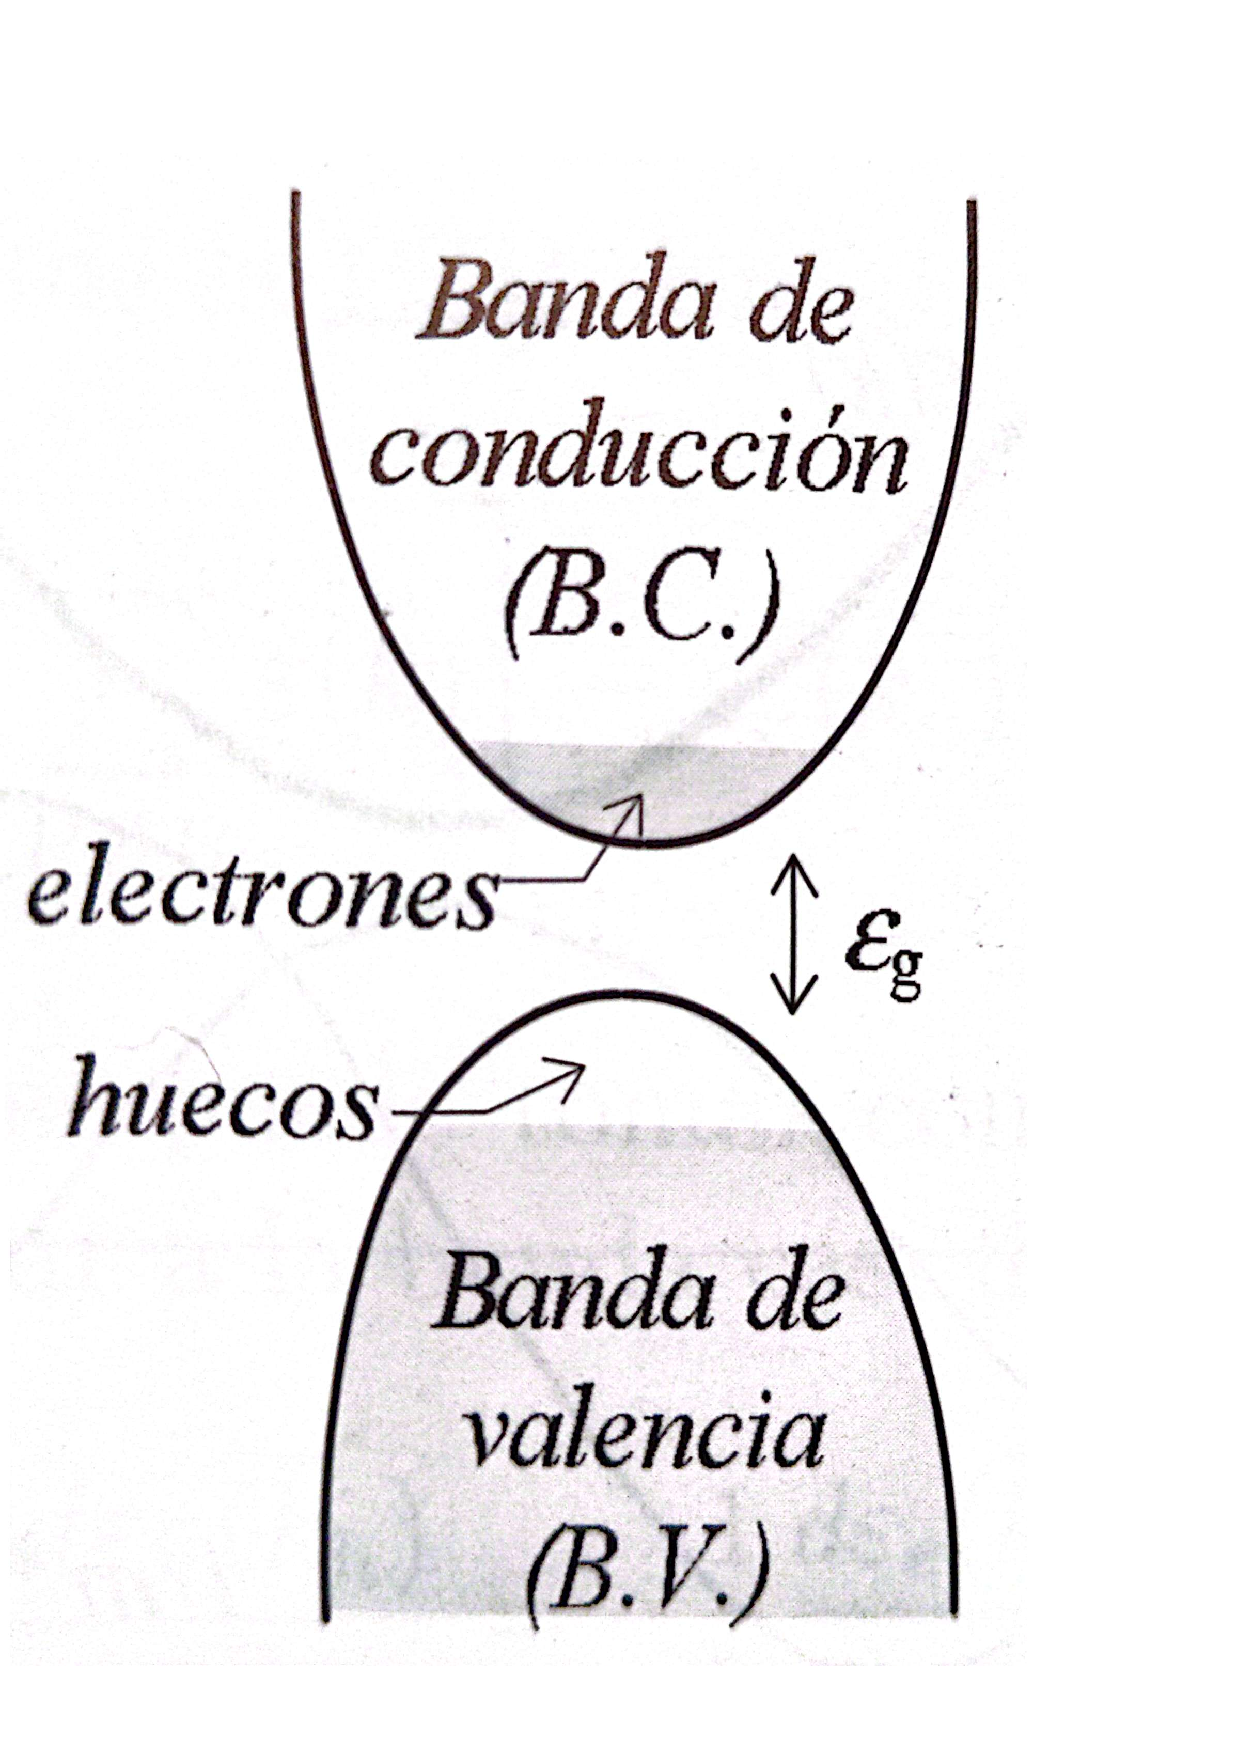
\includegraphics[scale=0.5]{Cuerpo/Ch_08/Fotos libro 1.pdf}
	\caption{}
	\label{Fig:08-01}
\end{figure}
\begin{figure}[h!] \centering
	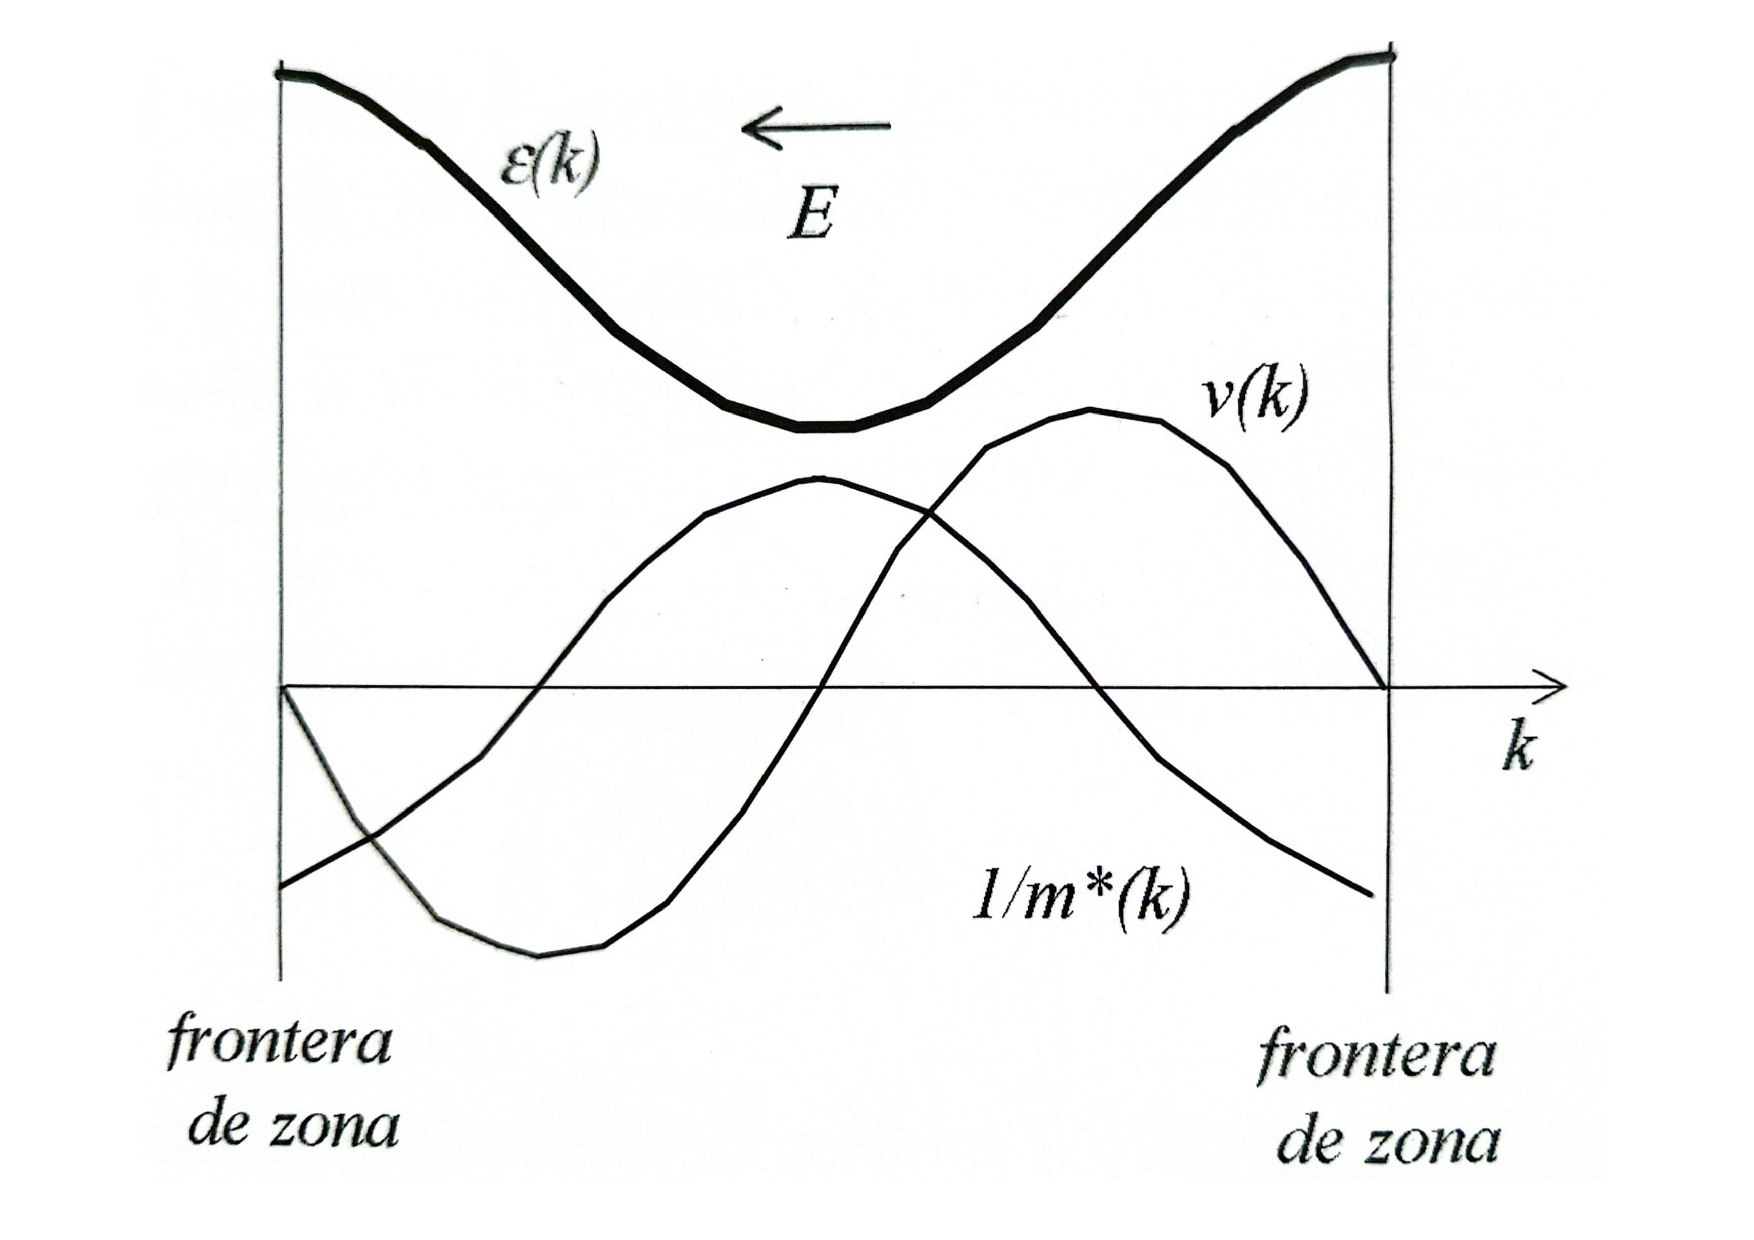
\includegraphics[scale=0.5]{Cuerpo/Ch_08/Fotos libro 2.pdf}
	\caption{}
	\label{Fig:08-02}
\end{figure}
\begin{figure}[h!] \centering
	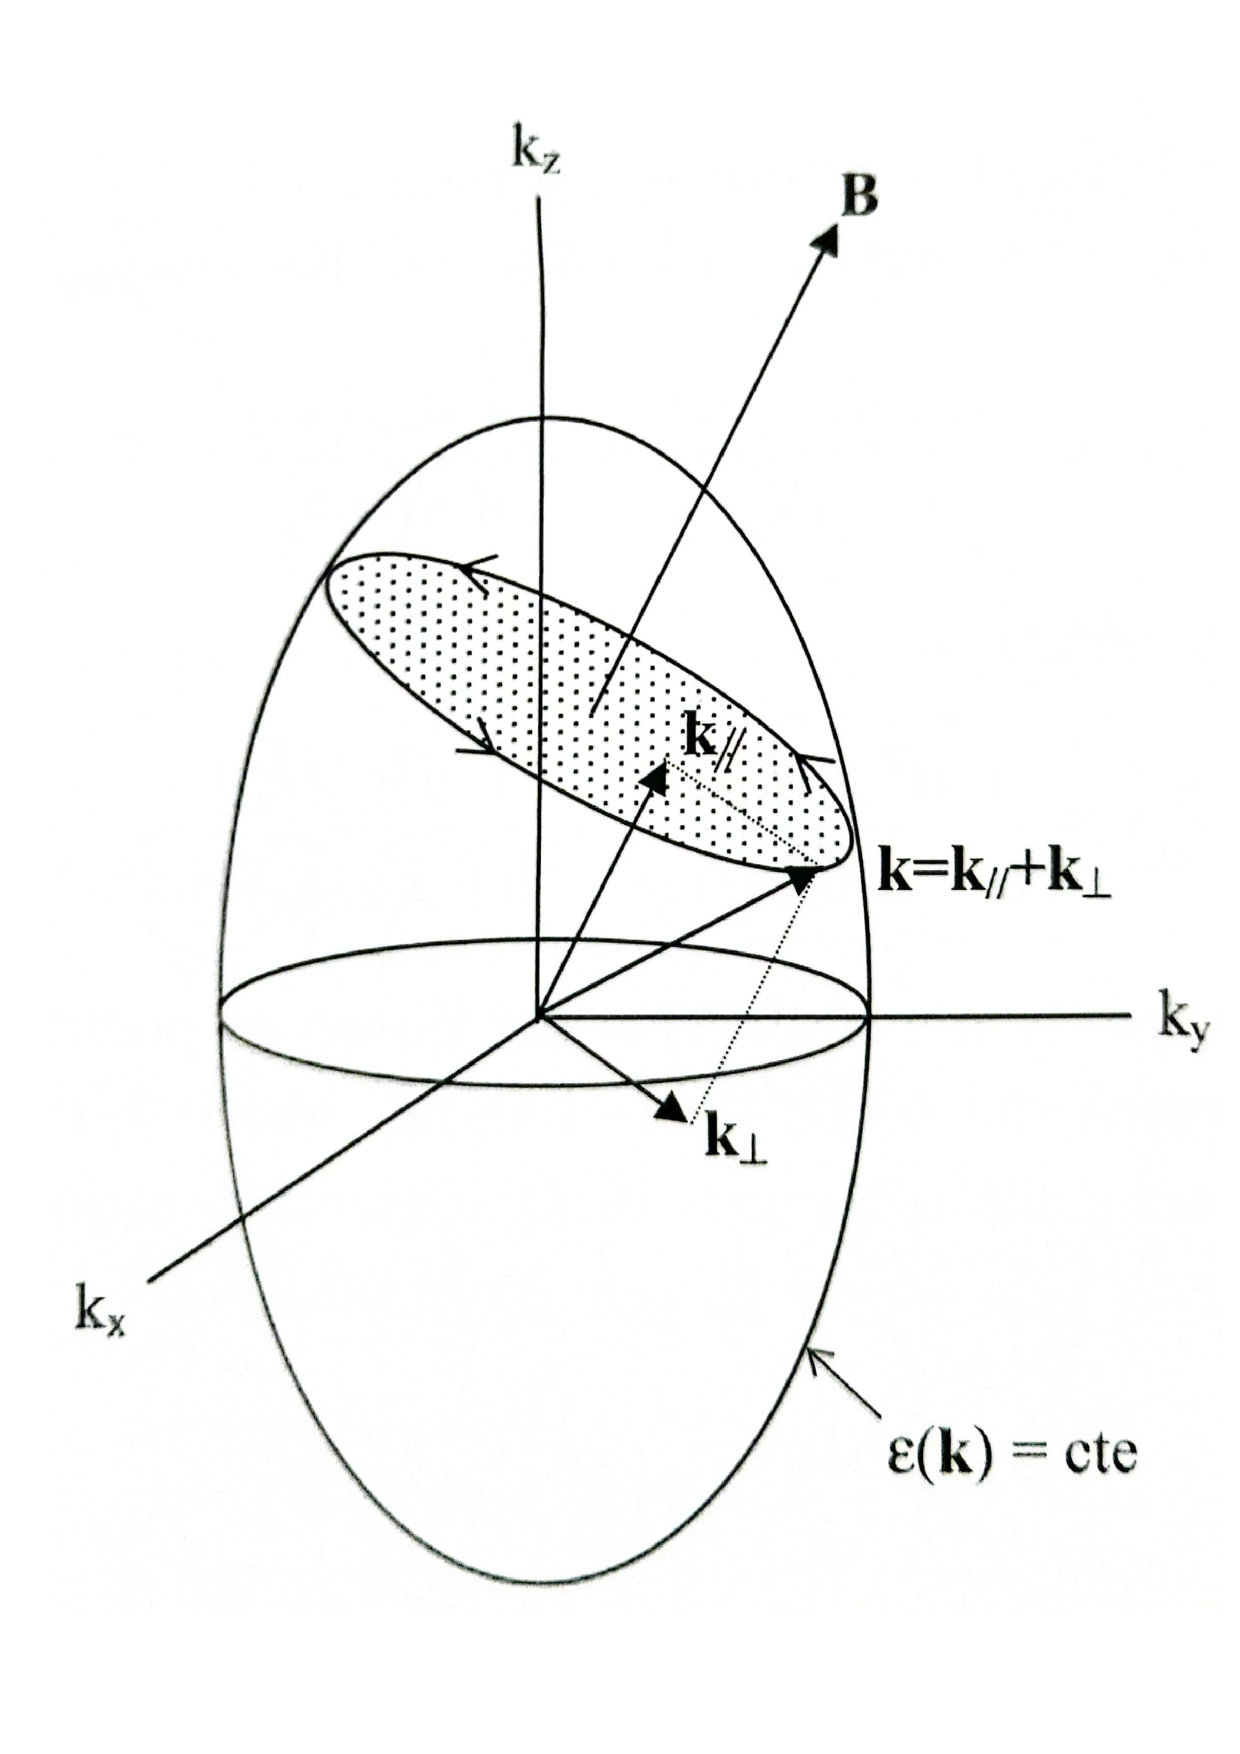
\includegraphics[scale=0.5]{Cuerpo/Ch_08/Fotos libro 3.pdf}
	\caption{}
	\label{Fig:08-03}
\end{figure}
\begin{figure}[h!] \centering
	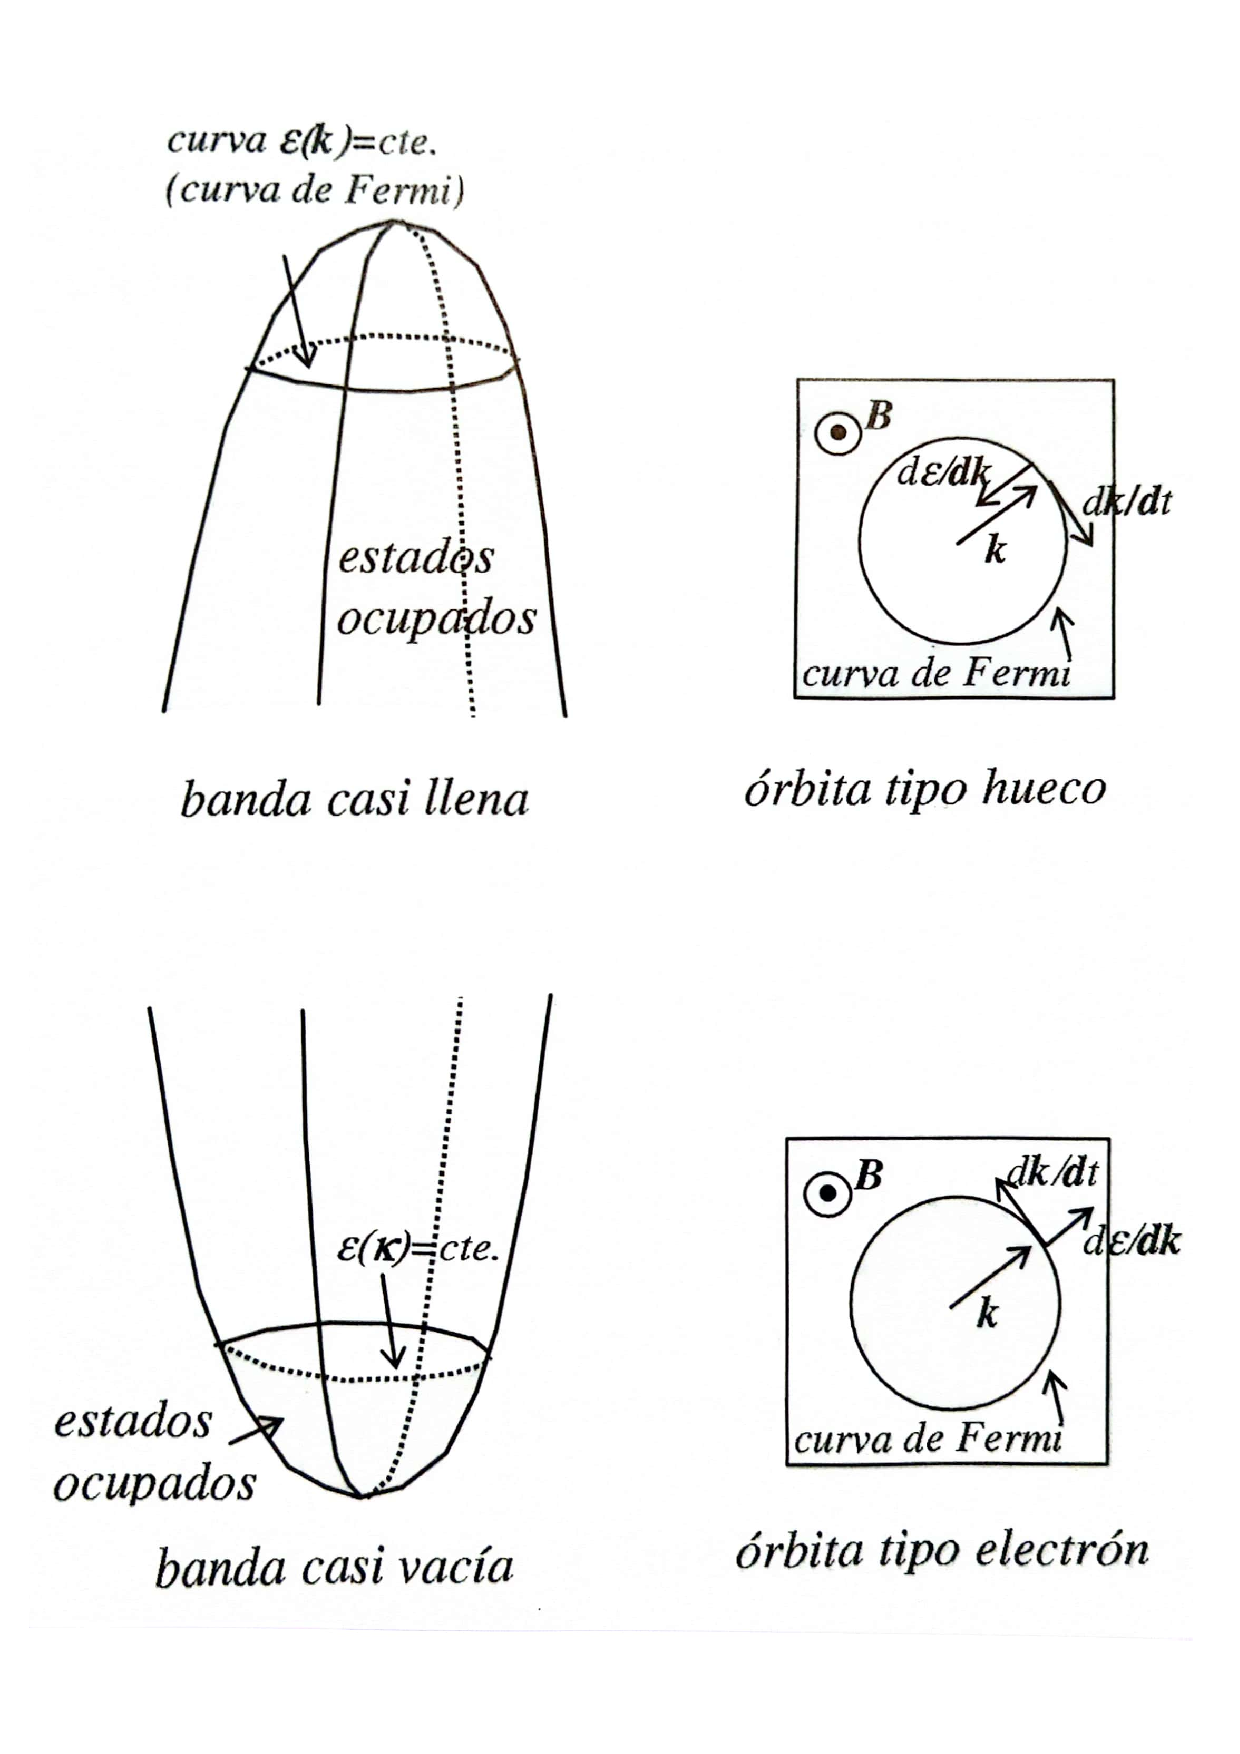
\includegraphics[scale=0.5]{Cuerpo/Ch_08/Fotos libro 4.pdf}
	\caption{}
	\label{Fig:08-04}
\end{figure}